% Social Event
\DeclareNewLayer[background, oddorevenpage, width=125mm,%
height=169mm, contents={%
  \vfill
  \begin{center}
    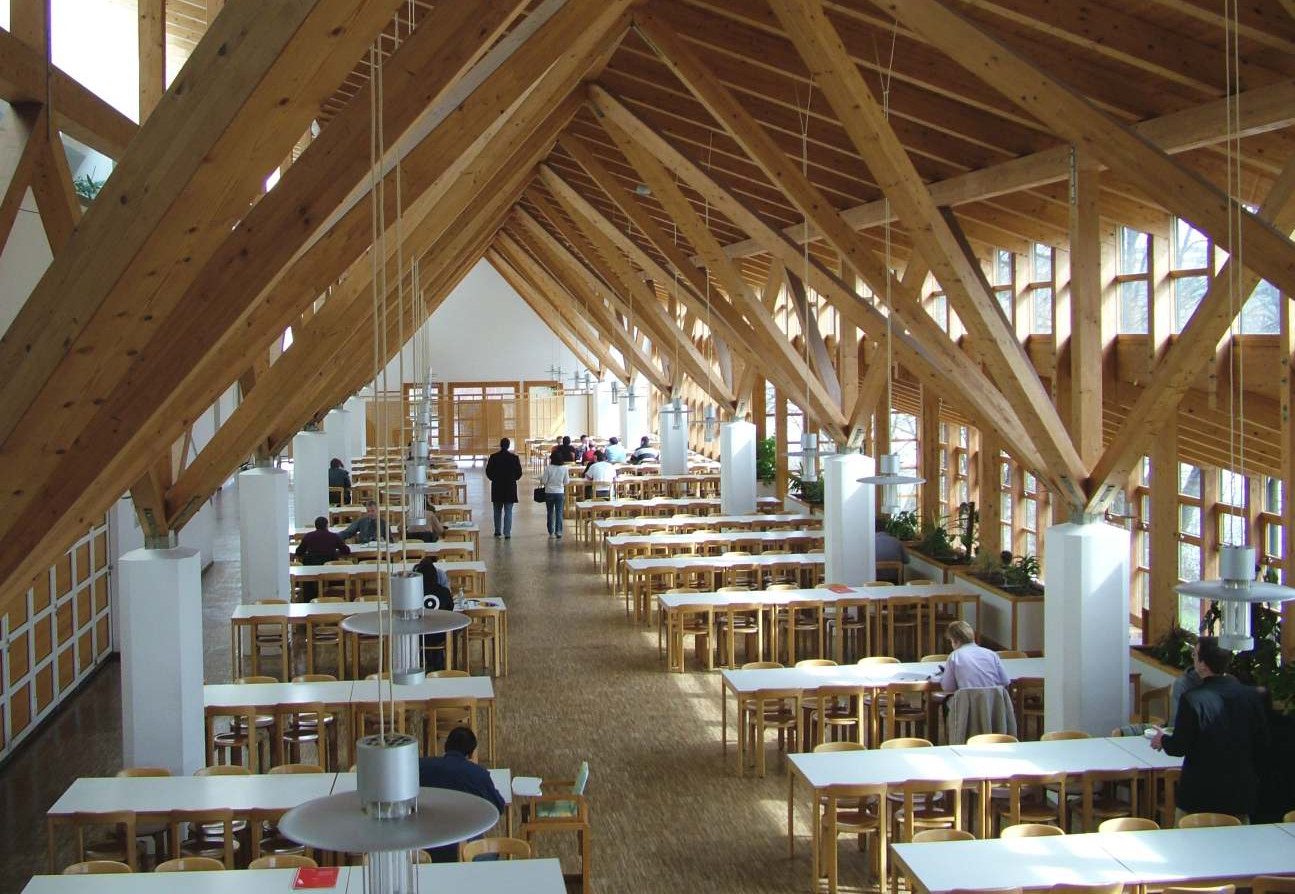
\includegraphics[width=115mm]{images-print/mensa.jpg}%
  \end{center}
}]{mensaevery}
\DeclareNewPageStyleByLayers[]{mensastyle}{cropmarksevery,mensaevery}
\newpage
\thispagestyle{mensastyle}
\section*{Dialoge am Inn}
\label{social-event}
Kontakte knüpfen und bekannte Gesichter wiedersehen, das ist jedes Jahr ein unverzichtbarer Teil der
FOSSGIS-Konferenz. Den besten Rahmen dafür bietet die Abendveranstaltung \emph{Dialoge am Inn} von 19:00
bis 23:00 Uhr. In der
direkt am grünen Ufer des Inns gelegenen Mensa der Uni Passau mit ihrer unverwechselbar offenen
Holz-Glas-Architektur ist gesellige Atmosphäre garantiert.

Die Teilnahme ist im
FOSSGIS-Konferenz-Ticket enthalten. Beim Buffet und dem reichhaltigen Getränkeangebot ist für jeden
Geschmack etwas dabei. Es wird um vorherige Anmeldung am Welcome Desk gebeten.
\newpage

\sponsorenbox{202_Camp2Camp.png}{0.4\textwidth}{4}{%
\textbf{Bronzesponsor\\Stand im EXPO-Forum}\\
Camptocamp gehört zu den führenden Schweizer Dienstleistern im Bereich von Open-Source-GIS
und ist durch sein Engagement in diversen Open-Source-Communitys international geschätzt.
Unsere Dienstleistungen stützen sich auf über 10 Jahre Erfahrung in der Umsetzung von innovativen (Web-)GIS-Lösungen
für Behörden und Unternehmen und erlauben einen hochwertigen und individuellen Service.}
\vfill
\sponsorenbox{210-beMasterGIS_final}{0.5\textwidth}{6}{%
\RaggedRight\textbf{Bronzesponsor\\Aussteller}\\
\justifying\noindent Online"=Masterstudiengang be\-Mas\-ter\-GIS\\
Fachanwender besit\-zen oft eine nur geringe GIS"=Ausbildung.
Seit 2010 hat sich der Online"=Masterstudiengang GIS an der HS Anhalt etabliert.
GIS-Anwender aus Verwaltungs-, Planungs-, Umwelt- oder Marketingumfeld studieren
berufsbegleitend in fünf Semestern überwiegend online mit wenigen Präsenzphasen.}

